%\documentclass[preprint,tightenlines,showpacs,showkeys,floatfix,
%nofootinbib,superscriptaddress,fleqn]{revtex4} 
\documentclass[tightenlines,floatfix,nofootinbib,superscriptaddress,fleqn]{revtex4-2} 
%\documentclass[aps,epsfig,tightlines,fleqn]{revtex4}
\usepackage{kotex}
\usepackage[HWP]{dhucs-interword}
\usepackage[dvips]{color}
\usepackage{graphicx}
\usepackage{bm}
%\usepackage{fancyhdr}
%\usepackage{dcolumn}
\usepackage{defcolor}
\usepackage{amsmath}
\usepackage{amsfonts}
\usepackage{amssymb}
\usepackage{amscd}
\usepackage{amsthm}
\usepackage[utf8]{inputenc}
%\pagestyle{fancy}
\usepackage{tikz}

\begin{document}

\title{\Large 2022년 2학기 물리학 II}
\author{김현철\footnote{Office: 5S-436D (면담시간 매주
    수요일-16:15$\sim$18:00)}} 
\email{hchkim@inha.ac.kr}
\affiliation{Hadron Theory Group, Department of Physics,
  Inha  University, Incheon 22212, Republic of Korea }
  \author{HuiJae-Lee} 
\email{hjlee6674@inha.edu}
\affiliation{Hadron Theory Group, Department of Physics,
  Inha  University, Incheon 22212, Republic of Korea }
\date{Autumn Semester, 2022}

\maketitle



\section*{\large Quiz 3}
\noindent {\bf 문제 1 [10pt].} 아래 질문에 답하세요.
\begin{itemize}
\item[(가)] 점전하가 만드는 전기장을 이용해서 가우스 법칙을 유도하세요.
\item[(나)] 도체 내부에서 전기장이 0이 됨을 설명하세요.
\item[(다)] 면전하밀도 $\sigma$로 대전되어 있고 무한히 큰 평면이 
  만드는 전기장의 크기는 $\sigma/2\varepsilon_0$입니다. 각각 양전하와
  음전하로 대전되어 있는 무한히 큰 평면 두 개가 거리 $d$ 만큼 떨어져서
  나란히 마주 보고 있을 때, 이 두 평면 사이에서 전기장을 구하세요. 
\end{itemize}
\vspace{0.5cm}

\noindent{\bf 풀이 : }
\begin{itemize}
  \item[(가)] 점전하의 전하를 $q$라 하고 이 점전하는 원점에 위치해 있다고 하자. 
  쿨롱의 법칙에 의해 이 점전하가 만드는 전기장 $\vec{E}$는
  \begin{align}
    \vec{E} = \frac{1}{4\pi\epsilon_0}\frac{q}{r^2}\hat{r}
  \end{align}
이다. 여기서 $\hat{r}$은 단위 벡터이다. 가우스 법칙을 유도하기 위해
중심이 원점이고 반지름이 $a$인 구를 통과하는 전기장의 플럭스 $\Phi_E$를 구해볼 것이다.
중심이 원점이고 반지름이 $a$인 구에 대해 면적분하여 구를 통과하는 전기장 $\vec{E}$의 
플럭스 $\Phi_E$는 정의에 의해 
\begin{align}\label{eq:1-1}
  \Phi_E=\oint \vec{E}\,d\vec{A}
\end{align}
으로 쓸 수 있다. $d\vec{A}$는 구에 대한 미소 면적으로 구면 좌표계를 도입하여 쓰면
\begin{align}
  d\vec{A} = a^2\sin\theta\,d\theta d\phi\,\hat{r}
\end{align}
이다. $\theta$는 $\hat{r}$과 $z$축이 이루는 각도이고 $\phi$는 $\hat{r}$을 $xy$평면에 정사영
내린 것과 $x$축이 이루는 각도이다. 적분범위는 구를 이루어야 하므로 $0<\theta<\pi$, 
$0<\phi<2\pi$이다. 따라서 플럭스 $\Phi_E$에 대한 식~(\ref{eq:1-1})는 다음과 같이
계산할 수 있다.
\begin{align}
  \begin{split}
    \Phi_E&=\int^{2\pi}_0\int^{\pi}_0 \frac{1}{4\pi\epsilon_0}\frac{q}{a^2}
    a^2\sin{\theta}\,d\theta d\phi\,(\hat{r}\cdot\hat{r})
    =\frac{q}{4\pi\epsilon_0}\left(\int^{2\pi}_0d\phi\right)
    \left(\int^{\pi}_0\sin{\theta}\,d\theta \right) \\
    &=\frac{q}{4\pi\epsilon_0}(2\pi)(2)=\frac{q}{\epsilon_0}.  
  \end{split}
\end{align}
이것이 가우스 법칙이다.
  \item[(나)] 도체에는 수많은 자유전자들이 존재하는데 자유전자들은 전기력에 의해 서로에게
  척력을 작용한다. 자유전자들이 서로를 밀어내기 때문에 모든 자유전자들은 결국 표면에 존재하게 되어
  도체 내부의 전기력은 $0$이 된다.
  \item[(다)] 
\begin{figure}[htbp]
  \centering
  \begin{tikzpicture}
    \draw[-latex] (0,0)--(0,1.2) node[above]{$y$};
    \draw[-latex] (0,0)--(1.2,0) node[above]{$x$};
    
    \draw (-3, 1)--(3, 1) node[right]{$+\sigma$};
    \draw (-3,-1)--(3,-1) node[right]{$-\sigma$};
    \draw[|<->|] (-4,-1)--(-4,1) node[below=25,left]{$d$};

    \draw[|<->|] (-1,-1.4)--( 1,-1.4) node[below=5,left=20]{$2r$};
    \draw[dashed,red] ( 1, 0.8)--( 1,-0.8);
    \draw[dashed,red] (-1, 0.8)--(-1,-0.8);
    \draw[dashed,red] (-1,-0.8)--( 1,-0.8);
    \draw[dashed,red] (-1, 0.8)--( 1, 0.8);
  \end{tikzpicture}
  \caption{면전하밀도 $\sigma$로 대전되어 있는 무한히 큰 두 평면}
  \label{fig:1-1}
\end{figure}
중심축이 각 평면에 수직이고 밑변의 반지름이 $r$인 원통을 생각하자. 이 원통의
표면을 가우스면으로 하여 가우스 법칙을 이용해 전기장을 구할 것이다. 먼저 전기장의 방향을
생각해보자. 도체의 전기장은 항상 표면의 수직된 방향이므로 평면 사이 공간에서 평면과 평행한
방향의 전기장은 존재하지 않는다. 즉, $x$방향의 전기장은 존재하지 않는다. 가우스면을 세 부분으로
나누어보자. 반지름이 $r$인 원형의 면이 위, 아래로 있어 이 면들을 각각 $A_{t}$, $A_{b}$이라
하고 원통의 옆면을 $A_s$
\end{itemize}


\vspace{0.5cm}
\noindent {\bf 문제 2 [10pt].} 한 모서리의 길이가 1.40 m인 정육면체가
그림~\ref{fig:1}처럼 균일한 전기장 아래 놓여있다. 만약 전기장이
N/C의 단위로 

\begin{figure}[htp]
  \centering
  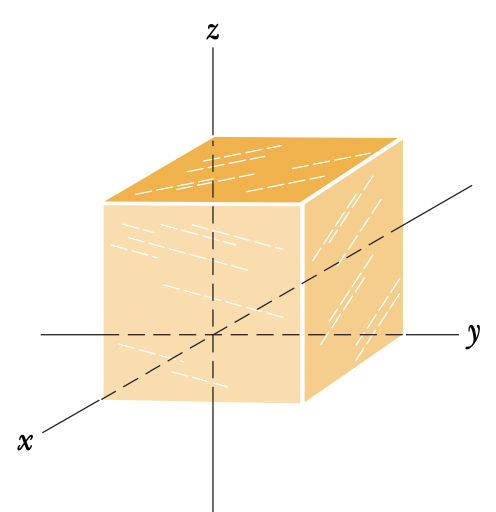
\includegraphics[scale=0.6]{qfig3-1.png}
  \caption{\textbf{문제 2}}
  \label{fig:1}
\end{figure}
\begin{itemize}
\item[(가)] $6.00\,\hat{\bm{i}}$,
\item[(나)] $-2.00\,\hat{\bm{j}}$,
\item[(다)] $-3.00\,\hat{\bm{i}}+4.00\,\hat{\bm{j}}$  
  라면 오른쪽 면을 통과하는 전기장 다발은 각각 얼마인가?
\item[(라)] 정육면체를 통과하는 알짜 전기장 다발(net electric flux)을
  구하여라.   
\end{itemize}
\vspace{0.5cm}

\noindent{\bf 풀이 : }
플럭스의 정의로부터 오른쪽 면에 대한 면벡터를 $\vec{A}$라 하면 
오른쪽 면을 통과하는 플럭스 $\Phi_E$와 면벡터 $\vec{A}$는
\begin{align}
  \Phi_E = \vec{E}\cdot\vec{A},\,\,\,
  \vec{A}=(1.40~\mathrm{m})^2\,\hat{\bm{j}}
\end{align}
이다. 
\begin{itemize}
  \item[(가)]$\vec{E} =  6.00~\mathrm{N/C}\,\hat{\bm{i}}$이므로 플럭스 $\Phi_E$는
  \begin{align}
    \Phi_E =(6.00~\mathrm{N/C})(1.40~\mathrm{m})^2(\hat{\bm{j}}\cdot\hat{\bm{i}})
    =\vec{0}
  \end{align}
  이다.
  \item[(나)]$\vec{E} = -2.00~\mathrm{N/C}\,\hat{\bm{j}}$이므로 플럭스 $\Phi_E$는
  \begin{align}
    \Phi_E =-(2.00~\mathrm{N/C})(1.40~\mathrm{m})^2(\hat{\bm{j}}\cdot\hat{\bm{j}})
    =3.92~\mathrm{N\cdot m^2/C}
  \end{align}
  이다.
  \item[(다)]$\vec{E} = [-3.00\,\hat{\bm{i}}+4.00\,\hat{\bm{j}}]~\mathrm{N/C}$이므로 
  플럭스 $\Phi_E$는
  \begin{align}
    \begin{split}
      \Phi_E &=-(3.00~\mathrm{N/C})(1.40~\mathrm{m})^2(\hat{\bm{j}}\cdot\hat{\bm{i}})
      +(4.00~\mathrm{N/C})(1.40~\mathrm{m})^2(\hat{\bm{j}}\cdot\hat{\bm{j}})  \\
      &=7.84~\mathrm{N\cdot m^2/C}
    \end{split}
  \end{align}
  이다.
  \item[(라)] 일반적인 전기장 $E_x\,\hat{\bm{i}}+E_y\,\hat{\bm{j}}+E_z\,\hat{\bm{k}}$와
  정육면체의 6개 면에 대응되는 면벡터 $\vec{A}_{\pm x},\,\vec{A}_{\pm y},
  \,\vec{A}_{\pm z}$을 이용하여 플럭스 $\Phi_E$를 생각해보자. 예를 들어, 면벡터 
  $\vec{A}_{+x}$와 $\vec{A}_{-z}$는
  \begin{align}
    \vec{A}_{+x} =  (1.40~\mathrm{m})^2\,\hat{\bm{i}},\,\,\,
    \vec{A}_{-z} = -(1.40~\mathrm{m})^2\,\hat{\bm{k}}
  \end{align}
  이다. 따라서 정육면체를 통과하는 알짜 전기장 다발, 모든 플럭스의 합 $\sum\Phi_E$은
  \begin{align}
    \sum\Phi_E=\vec{E}\cdot\vec{A}_{+x}+\vec{E}\cdot\vec{A}_{-x}
    +\vec{E}\cdot\vec{A}_{+y}+\vec{E}\cdot\vec{A}_{-y}
    +\vec{E}\cdot\vec{A}_{+z}+\vec{E}\cdot\vec{A}_{-z}
  \end{align}
  라고 할 수 있는데 전기장이 일정하므로 
  \begin{align}\label{eq:2-2}
    \sum\Phi_E=\vec{E}\cdot\left(\vec{A}_{+x}+\vec{A}_{-x}
    +\vec{A}_{+y}+\vec{A}_{-y}+\vec{A}_{+z}+\vec{A}_{-z}\right)
  \end{align}
  로 쓸 수 있다. 전기장이 일정하지 않았다면 각 면을 통과하는 전기장의 크기가 달랐을 것이므로
  위와 같이 쓸 수 없다. 그런데, 서로 평행한 면의 면벡터는 크기가 같고 방향이 반대이다. 즉,
  \begin{align}
    \vec{A}_{+x}=-\vec{A}_{-x},\,\,\,
    \vec{A}_{+y}=-\vec{A}_{-y},\,\,\,
    \vec{A}_{+z}=-\vec{A}_{-z}
  \end{align}
  이므로 식~(\ref{eq:2-2})의 면벡터의 합은 $0$이 된다. 따라서 
  알짜 전기장 다발 $\sum\Phi_E$은 $0$이다.
  \begin{align}
    \sum\Phi_E = 0.
  \end{align}
\end{itemize}
\vspace{0.5cm}
\noindent {\bf 문제 3 [20pt].} 그림~\ref{fig:2}처럼 질량이 1 mg이고
전하가 $q=2.0\times 10^{-8}$ C로 균일하게 분포되어 있는 작은 부도체
공이 얆고 전하가 균일하게 대전된 부도체 면과 $\theta=30^\circ$의
각을 이루며 부도체 실에 매달려 있다.  
\begin{figure}[htp]
  \centering
  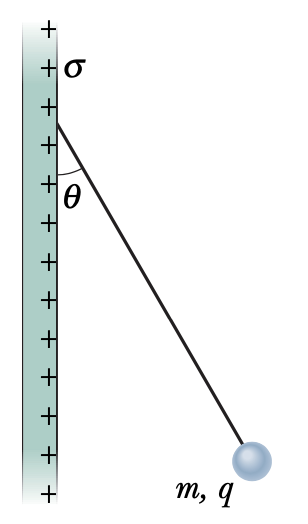
\includegraphics[scale=0.6]{qfig3-2.png}
  \caption{\textbf{문제 3}}
  \label{fig:2}
\end{figure}
이 절연체 판이 무한히 크다고 가정하자. 이와 같은 평형을 만들 수 있는
면전하밀도 $\sigma$를 구하여라.
\vspace{0.5cm}

\noindent{\bf 풀이 : } 
\begin{figure}
  \begin{tikzpicture}
    \draw (-2.5,0) -- (2.5,0) node [above] {$+x$};
    \draw (0,-2.5) -- (0,2.5) node [right] {$+y$};
    \draw [rotate=120,violet,very thick,-latex] (0.1,0) -- (2.2,0) 
    node [above,black] {$T$};
    
    \draw [red,very thick,-latex] (0.1,0) -- (1.6,0) 
    node [above,black] {$F_e$};

    \draw [blue,very thick,-latex] (0,-0.1) -- (0,-1.4) 
    node [right,black] {$F_g$};
  \end{tikzpicture} \caption{자유 물체 다이어그램}
\end{figure}

우선 부도체 공에 대한 자유 물체 다이어그램을 그려보자.
$T$는 장력, $F_g$는 공에 작용하는 중력이고 $F_e$는 절연체 판에 의해 공에 작용하는 
전기력이다. 공의 운동방정식은 다음과 같다.
\begin{align}
  \label{eq:3-1}\sum F_x &= F_e - T\sin\theta  ,\,\,\, \\
  \label{eq:3-2}\sum F_y &= T\cos\theta - F_g.
\end{align}
무한히 큰 판에 의한 전기장의 크기 $E$는
\begin{align}
  E=\frac{\sigma}{2\epsilon_0}
\end{align}
이고 공에 작용하는 전기력 $F_e$는
\begin{align}
  F_e = qE = \frac{q\sigma}{2\epsilon_0}
\end{align}
이다. 이를 $x$방향 운동방정식~(\ref{eq:3-1})에 대입하면
\begin{align}\label{eq:3-3}
  \frac{q\sigma}{2\epsilon_0}-T\sin\theta=0
\end{align}
을 얻는다. 이 식에서 장력 $T$만 구하면 면전하밀도 $\sigma$를 구할 수 있다. 
$y$방향 운동방정식~(\ref{eq:3-2})으로부터 장력 $T$를 다른 변수들로 표현하고
\begin{align}
  T\cos\theta = F_g \Longrightarrow T=\frac{mg}{\cos\theta}
\end{align}
이를 식~(\ref{eq:3-3})에 대입하면
\begin{align}
  \frac{q\sigma}{2\epsilon_0}-mg\tan\theta=0  \Longrightarrow
  \sigma = \frac{2\epsilon_0mg}{q}\tan\theta
\end{align}
으로 면전하밀도 $\sigma$에 대한 식을 얻는다. 공의 질량 $m$은 $1~\mathrm{mg}
=1\times 10^{-6}~\mathrm{kg}$이므로 면전하밀도 $\sigma$는
\begin{align}
  \begin{split}
    \sigma &= \frac{2(8.85\times 10^{-12}~\mathrm{C^2/N\cdot m^{2}})
    (1\times 10^{-6}~\mathrm{kg})
    (9.81~\mathrm{m/s^2})}
    {2.0\times 10^{-8}~\mathrm{C}}\tan 30^\circ \\
    &= 5.01~\mathrm{C/m^2}
  \end{split}
\end{align}
이다. 즉, 평형을 만들 수 있는 면전하밀도 $\sigma$는 $5.01~\mathrm{C/m^2}$이다.
\vspace{0.5cm}

\noindent {\bf 문제 4 [50pt].} 그림~\ref{fig:3}에서 상자 모양의 가우스
면이 $+24.0\varepsilon_0$ C의 알짜전하를 포함하고 전기장
$\vec{E}=[(10.0 + 2.00x)\,\hat{\bm{i}}-3.00\,\hat{\bm{j}}+
  bz\,\hat{\bm{k}}]$ N/C 안에 놓여 있다. 
\begin{figure}[htp]
  \centering
  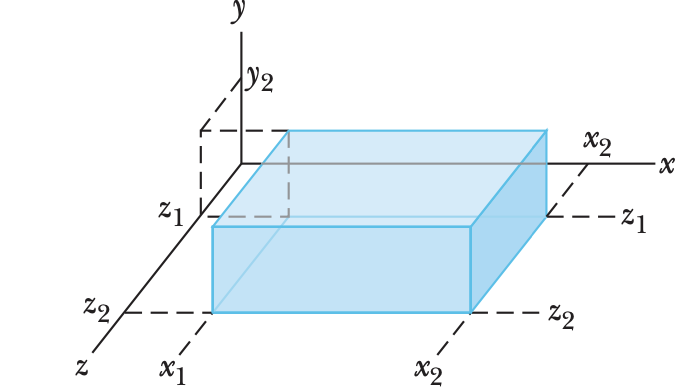
\includegraphics[scale=0.6]{qfig3-3.png}
  \caption{\textbf{문제 4}}
  \label{fig:3}
\end{figure}
$x$, $z$은 미터 단위로
  주어지고, $b$는 상수이다. 밑면은 $xz$평면이고, 윗면은 $y_2=1.00$ m를
  지나는 수평면이다. $x_1=1.00$ m, $x_2=4.00$ m, $z_1= 1.00$ m,
  $z_2=3.00$ m일 때, 상수 $b$는 얼마인가? 
\vspace{0.5cm}

\noindent{\bf 풀이 : } 가우스 법칙에 의하면 페곡면을 지나는 플럭스의 총합은 내부 전하량에
비례한다:
\begin{align}\label{eq:4-1}
  \int \vec{E}\cdot\,d\vec{A} = \frac{q_{in}}{\epsilon_0}.
\end{align}
이 경우는 전기장이 $x$와 $z$에 의존하므로 각 면에 대한 플럭스를 하나씩 구해야 한다.
직육면체에 존재하는 면 6개에 대응하는 면벡터를 각각 $\vec{A}_{\pm x}$, 
$\vec{A}_{\pm y}$, $\vec{A}_{\pm z}$라 하자. 예를 들어 $\vec{A}_{+x}$와
$\vec{A}_{-z}$는 각각
\begin{align}
  \begin{split}
    \vec{A}_{+x} &= \left.\left(y_2-y_1\right)\left(z_2-z_1\right)\right|_{x=x_2}
    \,\hat{\bm{i}}
    =[2.00\,\hat{\bm{i}}]~\mathrm{m^2}  \\
    \vec{A}_{-z} &= -\left.\left(x_2-x_1\right)\left(y_2-y_1\right)\right|_{z=z_1}
    \,\hat{\bm{k}}
    =[-3.00\,\hat{\bm{k}}]~\mathrm{m^2}
  \end{split}
\end{align}
이다. 또한 각 면벡터는 해당 방향 성분의 전기장과만 연산이 된다. 즉,
\begin{align}
  \int \vec{E}\cdot\,d\vec{A} = 
   \left(\int E_x\,d{A_{+x}}-\int E_x\,d{A_{-x}}\right)
  +\left(\int E_y\,d{A_{+y}}-\int E_y\,d{A_{-y}}\right)
  +\left(\int E_z\,d{A_{+z}}-\int E_z\,d{A_{-z}}\right)
\end{align}
을 계산하면 된다. $x$방향의 계산을 먼저 해보면
\begin{align}
  \begin{split}
    \int E_x\,d{A_{+x}}-\int E_x\,d{A_{-x}}
    &=\left.\int^{z_2}_{z_1}\int^{y_2}_{y_1} E_x\,dydz\right|_{x=x_2}
     -\left.\int^{z_2}_{z_1}\int^{y_2}_{y_1} E_x\,dydz\right|_{x=x_1} \\
    &=\left[\int^{3.00~\mathrm{m}}_{1.00~\mathrm{m}}
      \int^{1.00~\mathrm{m}}_{0~\mathrm{m}} 
      18.0\,dydz\right]~\mathrm{N/C}
    -\left[\int^{3.00~\mathrm{m}}_{1.00~\mathrm{m}}
    \int^{1.00~\mathrm{m}}_{0~\mathrm{m}} 
    12.0\,dydz\right]~\mathrm{N/C}  \\
    &=12.0~\mathrm{N/C}
  \end{split}
\end{align}
이므로 $x$방향으로 흐르는 플럭스의 총합은 $12~\mathrm{N/C}$이다. $y$방향의 계산은
\begin{align}
  \begin{split}
    \int E_y\,d{A_{+y}}-\int E_y\,d{A_{-y}}
    &=\left.\int^{z_2}_{z_1}\int^{x_2}_{x_1} E_y\,dxdz\right|_{y=y_2}
     -\left.\int^{z_2}_{z_1}\int^{x_2}_{x_1} E_y\,dxdz\right|_{y=y_1} \\
    &=-\left[\int^{3.00~\mathrm{m}}_{1.00~\mathrm{m}}
    \int^{4.00~\mathrm{m}}_{1.00~\mathrm{m}} 
    3.00\,dxdz\right]~\mathrm{N/C}
    +\left[\int^{3.00~\mathrm{m}}_{1.00~\mathrm{m}}
    \int^{4.00~\mathrm{m}}_{1.00~\mathrm{m}} 
    3.00\,dxdz\right]~\mathrm{N/C}  \\
    &=0~\mathrm{N/C}
  \end{split}
\end{align}
이다. 이는 $y$방향으로 흐르는 플럭스의 총합은 모두 상쇄되기 때문이다. $z$방향의 계산은
\begin{align}
  \begin{split}
    \int E_z\,d{A_{+z}}-\int E_z\,d{A_{-z}}
    &=\left.\int^{x_2}_{x_1}\int^{y_2}_{y_1} E_z\,dxdy\right|_{z=z_2}
     -\left.\int^{x_2}_{x_1}\int^{y_2}_{y_1} E_z\,dxdy\right|_{z=z_1} \\
    &=\left[\int^{1.00~\mathrm{m}}_{0~\mathrm{m}}
    \int^{4.00~\mathrm{m}}_{1.00~\mathrm{m}} 
    3.00b\,dxdy\right]~\mathrm{N/C}
  -\left[\int^{1.00~\mathrm{m}}_{0~\mathrm{m}}
  \int^{4.00~\mathrm{m}}_{1.00~\mathrm{m}} 
  1.00b\,dxdy\right]~\mathrm{N/C} \\
  &=6.00b~\mathrm{N/C}
  \end{split}
\end{align}
로 $z$방향으로 흐르는 플럭스의 총합이 $6.00b~\mathrm{N/C}$이라는 사실을 얻는다.
이 결과들과 직육면체 내부에 포함된 알짜전하 $+24.0\varepsilon_0$ C를 고려하여 
식~(\ref{eq:4-1})을 이용하면
\begin{align}
  12.0~\mathrm{N/C} + 0~\mathrm{N/C} + 6.00b~\mathrm{N/C}
  =24.0~\mathrm{N/C}
  \Longrightarrow b=2
\end{align}
와 같이 $b=2$를 얻는다.
\vspace{0.5cm}

\end{document}